% 足球顶点坐标的计算

\pentry{解三棱锥的两个重要公式} % 未完成

\begin{figure}[ht]
\centering
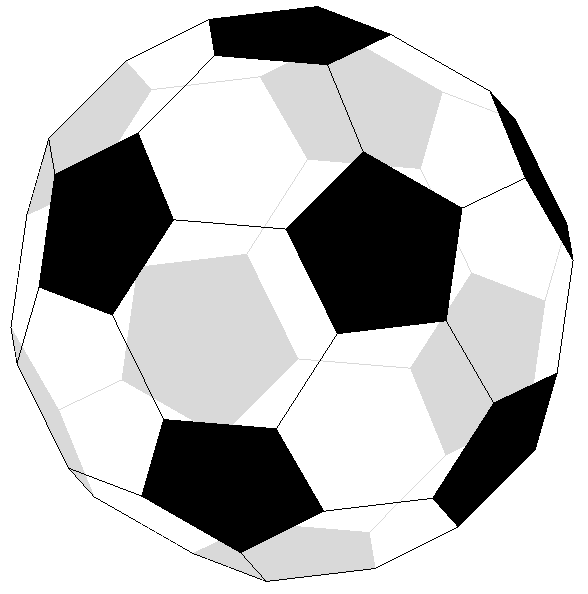
\includegraphics[width=5cm]{./figures/FootBl1.png}
\caption{足球透视图} \label{FootBl_fig1}
\end{figure}

足球的各种常用数据都可以由一个条件推出, 那就是它有 60 个顶点。 考虑到个顶点都有 3 条同样长度的棱, 棱的个数为
\begin{equation}
[\text{60 顶点}] \times [\text{3 条棱}] / [\text{每条棱有 2 个顶点}] = 90
\end{equation}
另外每个顶点都由一个正五边形和两个正六边形共用,所以五边形的个数为
\begin{equation}
[\text{60 顶点}] \times [\text{每个顶点 1 个五边形}] / [\text{每个五边形有 5 个顶点}] = 12
\end{equation}
同理, 六边形的个数为
\begin{equation}
[\text{60 顶点}] \times [\text{每个顶点 2 个六边形}] / [\text{每个六边形有 6 个顶点}] = 20
\end{equation}

\subsection{坐标计算}
以下所用到的方法不仅适用于足球, 还适用于其他多面体如正十二面体, 正二十面体等. 以足球的一个五边形作为底面, 得到足球的侧视图和俯视图如下(分别是左图与右图). 为了方便讨论, 我们根据这两个视图把足球的顶点按高度分为 A-H 这 8 层.并且逆时针给出相应的数字编号,详见侧视图和俯视图中的标注.

\begin{figure}[ht]
\centering
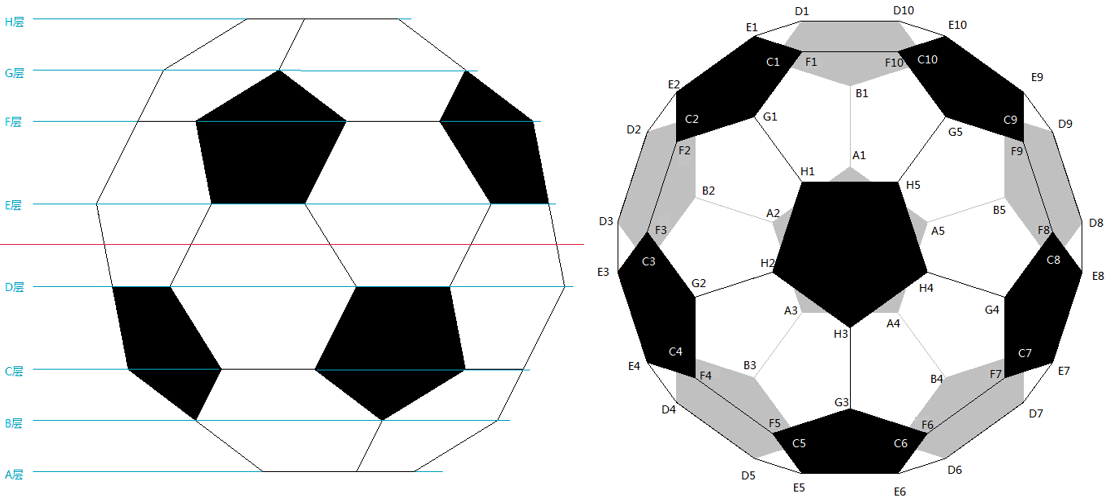
\includegraphics[width=14cm]{./figures/FootBl2.png}
\caption{各层和各顶点的命名} \label{FootBl_fig2}
\end{figure}

由于足球由正六边形和正五边形拼成, 足球的每一条棱都相等. 在以下计算中, 不妨设棱长为 1. 通过以下几个步骤, 就可以求解足球的各点的直角坐标.

\subsubsection{求出 $A_1$ 到 $A_5$ 的坐标}
直角坐标系中,令A层的五边形与XY平面重合,如下图.为了表示方便,令
\begin{equation}
S = \sin\frac{2\pi}{5} \qquad
C = \cos\frac{2\pi}{5} \qquad
s = \sin\frac{\pi}{5} \qquad
c = \cos\frac{\pi}{5}
\end{equation}
则点 $A_1$ 到 $A_5$ 的坐标分别为
\begin{equation}\label{FootBl_eq5}
\qty(0, \frac{1}{2s}, 0) \quad
\qty(-\frac{S}{2s}, \frac{C}{2s}, 0) \quad
\qty(-\frac12, -\frac{c}{2s}, 0) \quad
\qty(\frac12, -\frac{c}{2s}, 0) \quad
\qty(\frac{S}{2s}, \frac{C}{2s}, 0)
\end{equation}

\subsection{求出 $B_1$ 的坐标}
由解三棱锥的两个重要公式中的例2的方法, 可得线段 $B_2 A_2$ 与面 $A_1A_2A_3$ 的线面角(注意这里 $\gamma$ 的定义与 例2 中的 $\gamma$ 定义不同)
\begin{equation}
\gamma \approx 0.5536
\end{equation}
若把从 $A_1$ 指向 $A_2$ 的矢量记为 $\vec v_1$), $A_3$ 指向 $A_2$ 的矢量记为 $\vec v_2$, 将 $A_2$ 指向 $B_2$ 的矢量记为 $\vec u$, 可得
\begin{equation}
\vec u = \frac{\vec v_1 + \vec v_2}{\abs{\vec v_1 + \vec v_2}} \cos\gamma
+ \frac{\vec v_1 + \vec v_2}{\abs{\vec v_1 + \vec v_2}} \sin\gamma
= \frac{\sqrt{1 - 3S^2/4}}{2s} (\vec v_1 + \vec v_2) + \frac{\sqrt{3}}{2} (\vec v_2 + \vec v_1)
\end{equation}

由\autoref{FootBl_eq5} 得 $\vec v_1 = (-S, C-1, 0)/(2s)$, $\vec v_2 = (-S+s, C+c, 0)/(2s)$, 代入可得 $\vec u$ (结果略). 加上 $A_2$ 的坐标,可得 $B_2$ 的坐标. 接下来我们并不需要求出 B 层的其它坐标, 因为我们可以通过两个相当简单的公式依次求出剩下所有顶点的坐标。

\subsection{剩下所有顶点的坐标}
已知空间中多边形任意连续三点的坐标, 就可以求出第四个点的坐标。如果可以找到这种公式, 根据上文已求出的足球顶点就可以算出足球剩下的所有顶点的坐标。

例如(见\autoref{FootBl_fig2})根据已知的 $A_2, A_1, B_1$ 三个点,利用六边形公式可以算出 $C_1, C_2, B_2$. 根据 $A_2, A_3, B_2$ 又可以算出 $C_2, C_3, B_3$. 当 C 层完成后,又可以同理算出其他层。 下面推导这两个公式

\begin{figure}[ht]
\centering
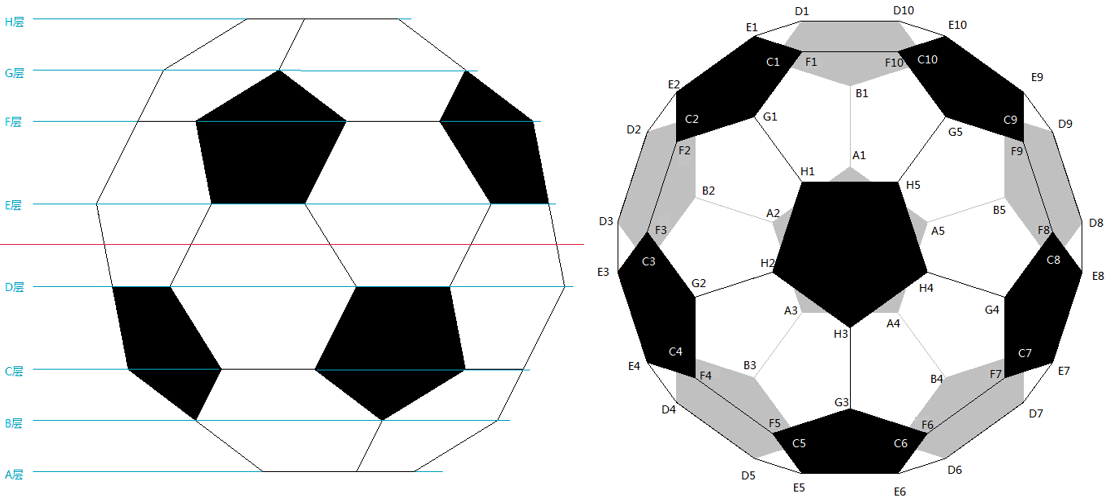
\includegraphics[width=14cm]{./figures/FootBl2.png}
\caption{由 5 边形的 3 个顶点坐标求第 4 个定点坐标} \label{FootBl_fig2}
\end{figure}

在正 $N$ 边形中, 记任意连续 4 点的位置矢量为 $\vec r_1, \vec r_2, \vec r_3, \vec r_4$, 我们希望能用 $\vec r_1, \vec r_2, \vec r_3$ 表示 $\vec r_4$。 令 $\vec v_i = \vec r_{i+1} - \vec r_i$, 从\autoref{}(以 5 边形)中不难发现
\begin{equation}
\vec v_3 = -\vec v_1 + 2\cos\frac{2\pi}{N} \cdot \vec v_2
\end{equation}
即
\begin{equation}
\vec r_4 = \vec r_1 - \vec r_2 + \vec r_3 + 2\cos\frac{2\pi}{5} \cdot (\vec r_3  - \vec r_2)
\end{equation}







